% Options for packages loaded elsewhere
\PassOptionsToPackage{unicode}{hyperref}
\PassOptionsToPackage{hyphens}{url}
\documentclass[
]{article}
\usepackage{xcolor}
\usepackage[margin=1in]{geometry}
\usepackage{amsmath,amssymb}
\setcounter{secnumdepth}{5}
\usepackage{iftex}
\ifPDFTeX
  \usepackage[T1]{fontenc}
  \usepackage[utf8]{inputenc}
  \usepackage{textcomp} % provide euro and other symbols
\else % if luatex or xetex
  \usepackage{unicode-math} % this also loads fontspec
  \defaultfontfeatures{Scale=MatchLowercase}
  \defaultfontfeatures[\rmfamily]{Ligatures=TeX,Scale=1}
\fi
\usepackage{lmodern}
\ifPDFTeX\else
  % xetex/luatex font selection
\fi
% Use upquote if available, for straight quotes in verbatim environments
\IfFileExists{upquote.sty}{\usepackage{upquote}}{}
\IfFileExists{microtype.sty}{% use microtype if available
  \usepackage[]{microtype}
  \UseMicrotypeSet[protrusion]{basicmath} % disable protrusion for tt fonts
}{}
\makeatletter
\@ifundefined{KOMAClassName}{% if non-KOMA class
  \IfFileExists{parskip.sty}{%
    \usepackage{parskip}
  }{% else
    \setlength{\parindent}{0pt}
    \setlength{\parskip}{6pt plus 2pt minus 1pt}}
}{% if KOMA class
  \KOMAoptions{parskip=half}}
\makeatother
\usepackage{color}
\usepackage{fancyvrb}
\newcommand{\VerbBar}{|}
\newcommand{\VERB}{\Verb[commandchars=\\\{\}]}
\DefineVerbatimEnvironment{Highlighting}{Verbatim}{commandchars=\\\{\}}
% Add ',fontsize=\small' for more characters per line
\usepackage{framed}
\definecolor{shadecolor}{RGB}{248,248,248}
\newenvironment{Shaded}{\begin{snugshade}}{\end{snugshade}}
\newcommand{\AlertTok}[1]{\textcolor[rgb]{0.94,0.16,0.16}{#1}}
\newcommand{\AnnotationTok}[1]{\textcolor[rgb]{0.56,0.35,0.01}{\textbf{\textit{#1}}}}
\newcommand{\AttributeTok}[1]{\textcolor[rgb]{0.13,0.29,0.53}{#1}}
\newcommand{\BaseNTok}[1]{\textcolor[rgb]{0.00,0.00,0.81}{#1}}
\newcommand{\BuiltInTok}[1]{#1}
\newcommand{\CharTok}[1]{\textcolor[rgb]{0.31,0.60,0.02}{#1}}
\newcommand{\CommentTok}[1]{\textcolor[rgb]{0.56,0.35,0.01}{\textit{#1}}}
\newcommand{\CommentVarTok}[1]{\textcolor[rgb]{0.56,0.35,0.01}{\textbf{\textit{#1}}}}
\newcommand{\ConstantTok}[1]{\textcolor[rgb]{0.56,0.35,0.01}{#1}}
\newcommand{\ControlFlowTok}[1]{\textcolor[rgb]{0.13,0.29,0.53}{\textbf{#1}}}
\newcommand{\DataTypeTok}[1]{\textcolor[rgb]{0.13,0.29,0.53}{#1}}
\newcommand{\DecValTok}[1]{\textcolor[rgb]{0.00,0.00,0.81}{#1}}
\newcommand{\DocumentationTok}[1]{\textcolor[rgb]{0.56,0.35,0.01}{\textbf{\textit{#1}}}}
\newcommand{\ErrorTok}[1]{\textcolor[rgb]{0.64,0.00,0.00}{\textbf{#1}}}
\newcommand{\ExtensionTok}[1]{#1}
\newcommand{\FloatTok}[1]{\textcolor[rgb]{0.00,0.00,0.81}{#1}}
\newcommand{\FunctionTok}[1]{\textcolor[rgb]{0.13,0.29,0.53}{\textbf{#1}}}
\newcommand{\ImportTok}[1]{#1}
\newcommand{\InformationTok}[1]{\textcolor[rgb]{0.56,0.35,0.01}{\textbf{\textit{#1}}}}
\newcommand{\KeywordTok}[1]{\textcolor[rgb]{0.13,0.29,0.53}{\textbf{#1}}}
\newcommand{\NormalTok}[1]{#1}
\newcommand{\OperatorTok}[1]{\textcolor[rgb]{0.81,0.36,0.00}{\textbf{#1}}}
\newcommand{\OtherTok}[1]{\textcolor[rgb]{0.56,0.35,0.01}{#1}}
\newcommand{\PreprocessorTok}[1]{\textcolor[rgb]{0.56,0.35,0.01}{\textit{#1}}}
\newcommand{\RegionMarkerTok}[1]{#1}
\newcommand{\SpecialCharTok}[1]{\textcolor[rgb]{0.81,0.36,0.00}{\textbf{#1}}}
\newcommand{\SpecialStringTok}[1]{\textcolor[rgb]{0.31,0.60,0.02}{#1}}
\newcommand{\StringTok}[1]{\textcolor[rgb]{0.31,0.60,0.02}{#1}}
\newcommand{\VariableTok}[1]{\textcolor[rgb]{0.00,0.00,0.00}{#1}}
\newcommand{\VerbatimStringTok}[1]{\textcolor[rgb]{0.31,0.60,0.02}{#1}}
\newcommand{\WarningTok}[1]{\textcolor[rgb]{0.56,0.35,0.01}{\textbf{\textit{#1}}}}
\usepackage{graphicx}
\makeatletter
\newsavebox\pandoc@box
\newcommand*\pandocbounded[1]{% scales image to fit in text height/width
  \sbox\pandoc@box{#1}%
  \Gscale@div\@tempa{\textheight}{\dimexpr\ht\pandoc@box+\dp\pandoc@box\relax}%
  \Gscale@div\@tempb{\linewidth}{\wd\pandoc@box}%
  \ifdim\@tempb\p@<\@tempa\p@\let\@tempa\@tempb\fi% select the smaller of both
  \ifdim\@tempa\p@<\p@\scalebox{\@tempa}{\usebox\pandoc@box}%
  \else\usebox{\pandoc@box}%
  \fi%
}
% Set default figure placement to htbp
\def\fps@figure{htbp}
\makeatother
\setlength{\emergencystretch}{3em} % prevent overfull lines
\providecommand{\tightlist}{%
  \setlength{\itemsep}{0pt}\setlength{\parskip}{0pt}}
\usepackage[]{natbib}
\bibliographystyle{plainnat}
\usepackage{bookmark}
\IfFileExists{xurl.sty}{\usepackage{xurl}}{} % add URL line breaks if available
\urlstyle{same}
\hypersetup{
  pdftitle={Appendix B --- Longitudinal Analysis of Rating Growth (Lichess)},
  pdfauthor={Tina Huynh},
  hidelinks,
  pdfcreator={LaTeX via pandoc}}

\title{Appendix B --- Longitudinal Analysis of Rating Growth (Lichess)}
\author{Tina Huynh}
\date{2025-10-15}

\begin{document}
\maketitle

{
\setcounter{tocdepth}{2}
\tableofcontents
}
\subsection{Appendix B --- Longitudinal Analysis of Rating Growth
(Lichess)}\label{appendix-b-longitudinal-analysis-of-rating-growth-lichess}

\subsubsection{B.1 Data Acquisition}\label{b.1-data-acquisition}

\begin{Shaded}
\begin{Highlighting}[]
\FunctionTok{library}\NormalTok{(tidyverse)}
\FunctionTok{library}\NormalTok{(jsonlite)}
\FunctionTok{library}\NormalTok{(lubridate)}
\FunctionTok{library}\NormalTok{(httr)}

\CommentTok{\# Load random subset of users from the Lichess summary}
\NormalTok{lichess\_path }\OtherTok{\textless{}{-}} \StringTok{"../../data/lichess\_clean.csv"}
\NormalTok{lichess\_users }\OtherTok{\textless{}{-}} \FunctionTok{read\_csv}\NormalTok{(lichess\_path, }\AttributeTok{show\_col\_types =} \ConstantTok{FALSE}\NormalTok{) }\SpecialCharTok{\%\textgreater{}\%}
    \FunctionTok{slice\_sample}\NormalTok{(}\AttributeTok{n =} \DecValTok{15}\NormalTok{) }\SpecialCharTok{\%\textgreater{}\%} \CommentTok{\# pull 15 random users for plotting}
    \FunctionTok{pull}\NormalTok{(user)}

\CommentTok{\# Debug: Check selected users}
\FunctionTok{cat}\NormalTok{(}\StringTok{"Selected users:}\SpecialCharTok{\textbackslash{}n}\StringTok{"}\NormalTok{)}
\end{Highlighting}
\end{Shaded}

\begin{verbatim}
## Selected users:
\end{verbatim}

\begin{Shaded}
\begin{Highlighting}[]
\FunctionTok{print}\NormalTok{(lichess\_users)}
\end{Highlighting}
\end{Shaded}

\begin{verbatim}
##  [1] "snoozer"             "Kydravets-Mark19"    "Dark_Cast1gator"    
##  [4] "Daniil1007"          "Chess_Training_2021" "ManuDavid2910"      
##  [7] "wExoqtic"            "daaleksandrov"       "RakitinD"           
## [10] "Parakon1"            "Isaev_Anton_Val"     "Kotov_Syndrome"     
## [13] "IALIIALIIALI"        "lyxxj"               "Zhigalko_Sergei"
\end{verbatim}

\begin{Shaded}
\begin{Highlighting}[]
\CommentTok{\# Function to retrieve rating history for a given user}
\NormalTok{get\_rating\_history }\OtherTok{\textless{}{-}} \ControlFlowTok{function}\NormalTok{(username) \{}
    \FunctionTok{cat}\NormalTok{(}\FunctionTok{paste0}\NormalTok{(}\StringTok{"}\SpecialCharTok{\textbackslash{}n}\StringTok{Fetching data for user: "}\NormalTok{, username, }\StringTok{"}\SpecialCharTok{\textbackslash{}n}\StringTok{"}\NormalTok{))}
    \FunctionTok{Sys.sleep}\NormalTok{(}\FunctionTok{runif}\NormalTok{(}\DecValTok{1}\NormalTok{, }\FloatTok{0.5}\NormalTok{, }\FloatTok{1.2}\NormalTok{)) }\CommentTok{\# polite delay}
\NormalTok{    url }\OtherTok{\textless{}{-}} \FunctionTok{paste0}\NormalTok{(}\StringTok{"https://lichess.org/api/user/"}\NormalTok{, username, }\StringTok{"/rating{-}history"}\NormalTok{)}
    \FunctionTok{tryCatch}\NormalTok{(}
\NormalTok{        \{}
\NormalTok{            response }\OtherTok{\textless{}{-}} \FunctionTok{fromJSON}\NormalTok{(url, }\AttributeTok{simplifyDataFrame =} \ConstantTok{FALSE}\NormalTok{)}
            \FunctionTok{cat}\NormalTok{(}\FunctionTok{paste0}\NormalTok{(}\StringTok{"  Response length: "}\NormalTok{, }\FunctionTok{length}\NormalTok{(response), }\StringTok{"}\SpecialCharTok{\textbackslash{}n}\StringTok{"}\NormalTok{))}
            \ControlFlowTok{if}\NormalTok{ (}\FunctionTok{length}\NormalTok{(response) }\SpecialCharTok{==} \DecValTok{0}\NormalTok{) \{}
                \FunctionTok{cat}\NormalTok{(}\StringTok{"  No rating history available}\SpecialCharTok{\textbackslash{}n}\StringTok{"}\NormalTok{)}
                \FunctionTok{return}\NormalTok{(}\ConstantTok{NULL}\NormalTok{)}
\NormalTok{            \}}
            
            \CommentTok{\# Process each game type}
\NormalTok{            result\_list }\OtherTok{\textless{}{-}} \FunctionTok{list}\NormalTok{()}
            \ControlFlowTok{for}\NormalTok{ (i }\ControlFlowTok{in} \FunctionTok{seq\_along}\NormalTok{(response)) \{}
\NormalTok{                item }\OtherTok{\textless{}{-}}\NormalTok{ response[[i]]}
\NormalTok{                game\_type }\OtherTok{\textless{}{-}}\NormalTok{ item[[}\StringTok{"name"}\NormalTok{]]}
\NormalTok{                points\_data }\OtherTok{\textless{}{-}}\NormalTok{ item[[}\StringTok{"points"}\NormalTok{]]}
                
                \ControlFlowTok{if}\NormalTok{ (}\SpecialCharTok{!}\FunctionTok{is.null}\NormalTok{(points\_data) }\SpecialCharTok{\&\&} \FunctionTok{length}\NormalTok{(points\_data) }\SpecialCharTok{\textgreater{}} \DecValTok{0}\NormalTok{) \{}
                    \CommentTok{\# Handle different possible structures}
                    \ControlFlowTok{if}\NormalTok{ (}\FunctionTok{is.list}\NormalTok{(points\_data) }\SpecialCharTok{\&\&} \SpecialCharTok{!}\FunctionTok{is.data.frame}\NormalTok{(points\_data)) \{}
                        \CommentTok{\# Convert list of vectors to matrix}
\NormalTok{                        points\_matrix }\OtherTok{\textless{}{-}} \FunctionTok{matrix}\NormalTok{(}\FunctionTok{unlist}\NormalTok{(points\_data), }\AttributeTok{ncol =} \DecValTok{2}\NormalTok{, }\AttributeTok{byrow =} \ConstantTok{TRUE}\NormalTok{)}
\NormalTok{                    \} }\ControlFlowTok{else} \ControlFlowTok{if}\NormalTok{ (}\FunctionTok{is.matrix}\NormalTok{(points\_data)) \{}
\NormalTok{                        points\_matrix }\OtherTok{\textless{}{-}}\NormalTok{ points\_data}
\NormalTok{                    \} }\ControlFlowTok{else}\NormalTok{ \{}
                        \ControlFlowTok{next}  \CommentTok{\# Skip if unexpected format}
\NormalTok{                    \}}
                    
\NormalTok{                    result\_list[[i]] }\OtherTok{\textless{}{-}} \FunctionTok{tibble}\NormalTok{(}
                        \AttributeTok{user =}\NormalTok{ username,}
                        \AttributeTok{category =}\NormalTok{ game\_type,}
                        \AttributeTok{date\_index =}\NormalTok{ points\_matrix[, }\DecValTok{1}\NormalTok{],}
                        \AttributeTok{rating =}\NormalTok{ points\_matrix[, }\DecValTok{2}\NormalTok{]}
\NormalTok{                    ) }\SpecialCharTok{\%\textgreater{}\%}
                        \FunctionTok{mutate}\NormalTok{(}\AttributeTok{date =} \FunctionTok{as\_date}\NormalTok{(}\StringTok{"2013{-}01{-}01"}\NormalTok{) }\SpecialCharTok{+} \FunctionTok{weeks}\NormalTok{(date\_index))}
\NormalTok{                \}}
\NormalTok{            \}}
            
            \ControlFlowTok{if}\NormalTok{ (}\FunctionTok{length}\NormalTok{(result\_list) }\SpecialCharTok{\textgreater{}} \DecValTok{0}\NormalTok{) \{}
                \FunctionTok{return}\NormalTok{(}\FunctionTok{bind\_rows}\NormalTok{(result\_list))}
\NormalTok{            \} }\ControlFlowTok{else}\NormalTok{ \{}
                \FunctionTok{cat}\NormalTok{(}\StringTok{"  No valid rating points found}\SpecialCharTok{\textbackslash{}n}\StringTok{"}\NormalTok{)}
                \FunctionTok{return}\NormalTok{(}\ConstantTok{NULL}\NormalTok{)}
\NormalTok{            \}}
\NormalTok{        \},}
        \AttributeTok{error =} \ControlFlowTok{function}\NormalTok{(e) \{}
            \FunctionTok{cat}\NormalTok{(}\FunctionTok{paste0}\NormalTok{(}\StringTok{"  Error: "}\NormalTok{, e}\SpecialCharTok{$}\NormalTok{message, }\StringTok{"}\SpecialCharTok{\textbackslash{}n}\StringTok{"}\NormalTok{))}
            \FunctionTok{return}\NormalTok{(}\ConstantTok{NULL}\NormalTok{)}
\NormalTok{        \}}
\NormalTok{    )}
\NormalTok{\}}

\CommentTok{\# Collect rating histories}
\NormalTok{rating\_histories }\OtherTok{\textless{}{-}} \FunctionTok{map\_dfr}\NormalTok{(lichess\_users, get\_rating\_history)}
\end{Highlighting}
\end{Shaded}

\begin{verbatim}
## 
## Fetching data for user: snoozer
##   Response length: 15
## 
## Fetching data for user: Kydravets-Mark19
##   Response length: 15
## 
## Fetching data for user: Dark_Cast1gator
##   Response length: 15
## 
## Fetching data for user: Daniil1007
##   Response length: 15
## 
## Fetching data for user: Chess_Training_2021
##   Response length: 15
## 
## Fetching data for user: ManuDavid2910
##   Response length: 15
## 
## Fetching data for user: wExoqtic
##   Response length: 15
## 
## Fetching data for user: daaleksandrov
##   Response length: 15
## 
## Fetching data for user: RakitinD
##   Response length: 15
## 
## Fetching data for user: Parakon1
##   Response length: 15
## 
## Fetching data for user: Isaev_Anton_Val
##   Response length: 15
## 
## Fetching data for user: Kotov_Syndrome
##   Response length: 15
## 
## Fetching data for user: IALIIALIIALI
##   Response length: 15
## 
## Fetching data for user: lyxxj
##   Response length: 15
## 
## Fetching data for user: Zhigalko_Sergei
##   Response length: 15
\end{verbatim}

\begin{Shaded}
\begin{Highlighting}[]
\FunctionTok{write\_csv}\NormalTok{(rating\_histories, }\StringTok{"../../data/lichess\_rating\_history.csv"}\NormalTok{)}
\FunctionTok{glimpse}\NormalTok{(rating\_histories)}
\end{Highlighting}
\end{Shaded}

\begin{verbatim}
## Rows: 30,727
## Columns: 5
## $ user       <chr> "snoozer", "snoozer", "snoozer", "snoozer", "snoozer", "sno~
## $ category   <chr> "UltraBullet", "UltraBullet", "UltraBullet", "UltraBullet",~
## $ date_index <int> 2017, 2017, 2017, 2017, 2017, 2017, 2017, 2017, 2017, 2017,~
## $ rating     <int> 6, 6, 6, 6, 8, 9, 9, 9, 9, 9, 10, 10, 10, 10, 10, 10, 10, 1~
## $ date       <date> 2051-08-29, 2051-08-29, 2051-08-29, 2051-08-29, 2051-08-29~
\end{verbatim}

\begin{center}\rule{0.5\linewidth}{0.5pt}\end{center}

\subsubsection{B.2 Time-Series Cleaning and
Aggregation}\label{b.2-time-series-cleaning-and-aggregation}

\begin{Shaded}
\begin{Highlighting}[]
\CommentTok{\# Clean, filter, and aggregate by category (e.g., Blitz, Rapid)}
\NormalTok{rating\_summary }\OtherTok{\textless{}{-}}\NormalTok{ rating\_histories }\SpecialCharTok{\%\textgreater{}\%}
    \FunctionTok{filter}\NormalTok{(}\SpecialCharTok{!}\FunctionTok{is.na}\NormalTok{(rating)) }\SpecialCharTok{\%\textgreater{}\%}
    \FunctionTok{group\_by}\NormalTok{(user, category) }\SpecialCharTok{\%\textgreater{}\%}
    \FunctionTok{mutate}\NormalTok{(}
        \AttributeTok{rating\_smooth =}\NormalTok{ zoo}\SpecialCharTok{::}\FunctionTok{rollapply}\NormalTok{(rating, }\AttributeTok{width =} \DecValTok{3}\NormalTok{, }\AttributeTok{FUN =}\NormalTok{ mean, }\AttributeTok{fill =} \ConstantTok{NA}\NormalTok{, }\AttributeTok{align =} \StringTok{"right"}\NormalTok{),}
        \AttributeTok{relative\_time =} \FunctionTok{row\_number}\NormalTok{()}
\NormalTok{    ) }\SpecialCharTok{\%\textgreater{}\%}
    \FunctionTok{ungroup}\NormalTok{()}

\FunctionTok{head}\NormalTok{(rating\_summary)}
\end{Highlighting}
\end{Shaded}

\begin{verbatim}
## # A tibble: 6 x 7
##   user    category    date_index rating date       rating_smooth relative_time
##   <chr>   <chr>            <int>  <int> <date>             <dbl>         <int>
## 1 snoozer UltraBullet       2017      6 2051-08-29         NA                1
## 2 snoozer UltraBullet       2017      6 2051-08-29         NA                2
## 3 snoozer UltraBullet       2017      6 2051-08-29          6                3
## 4 snoozer UltraBullet       2017      6 2051-08-29          6                4
## 5 snoozer UltraBullet       2017      8 2051-08-29          6.67             5
## 6 snoozer UltraBullet       2017      9 2051-08-29          7.67             6
\end{verbatim}

\begin{center}\rule{0.5\linewidth}{0.5pt}\end{center}

\subsubsection{B.3 Visualization: Rating Progression Over
Time}\label{b.3-visualization-rating-progression-over-time}

\begin{Shaded}
\begin{Highlighting}[]
\FunctionTok{ggplot}\NormalTok{(rating\_summary, }\FunctionTok{aes}\NormalTok{(}\AttributeTok{x =}\NormalTok{ relative\_time, }\AttributeTok{y =}\NormalTok{ rating\_smooth, }\AttributeTok{color =}\NormalTok{ user)) }\SpecialCharTok{+}
    \FunctionTok{geom\_line}\NormalTok{(}\AttributeTok{linewidth =} \DecValTok{1}\NormalTok{) }\SpecialCharTok{+}
    \FunctionTok{facet\_wrap}\NormalTok{(}\SpecialCharTok{\textasciitilde{}}\NormalTok{category, }\AttributeTok{scales =} \StringTok{"free\_y"}\NormalTok{) }\SpecialCharTok{+}
    \FunctionTok{labs}\NormalTok{(}
        \AttributeTok{title =} \StringTok{"Lichess Rating Progression Over Time"}\NormalTok{,}
        \AttributeTok{subtitle =} \StringTok{"Sample of 5 Randomly Selected Users Across Game Categories"}\NormalTok{,}
        \AttributeTok{x =} \StringTok{"Sequential Game Weeks (relative index)"}\NormalTok{,}
        \AttributeTok{y =} \StringTok{"Smoothed Rating (3{-}period rolling mean)"}\NormalTok{,}
        \AttributeTok{color =} \StringTok{"User"}
\NormalTok{    ) }\SpecialCharTok{+}
    \FunctionTok{theme\_minimal}\NormalTok{(}\AttributeTok{base\_size =} \DecValTok{12}\NormalTok{)}
\end{Highlighting}
\end{Shaded}

\begin{verbatim}
## Warning: Removed 32 rows containing missing values or values outside the scale range
## (`geom_line()`).
\end{verbatim}

\pandocbounded{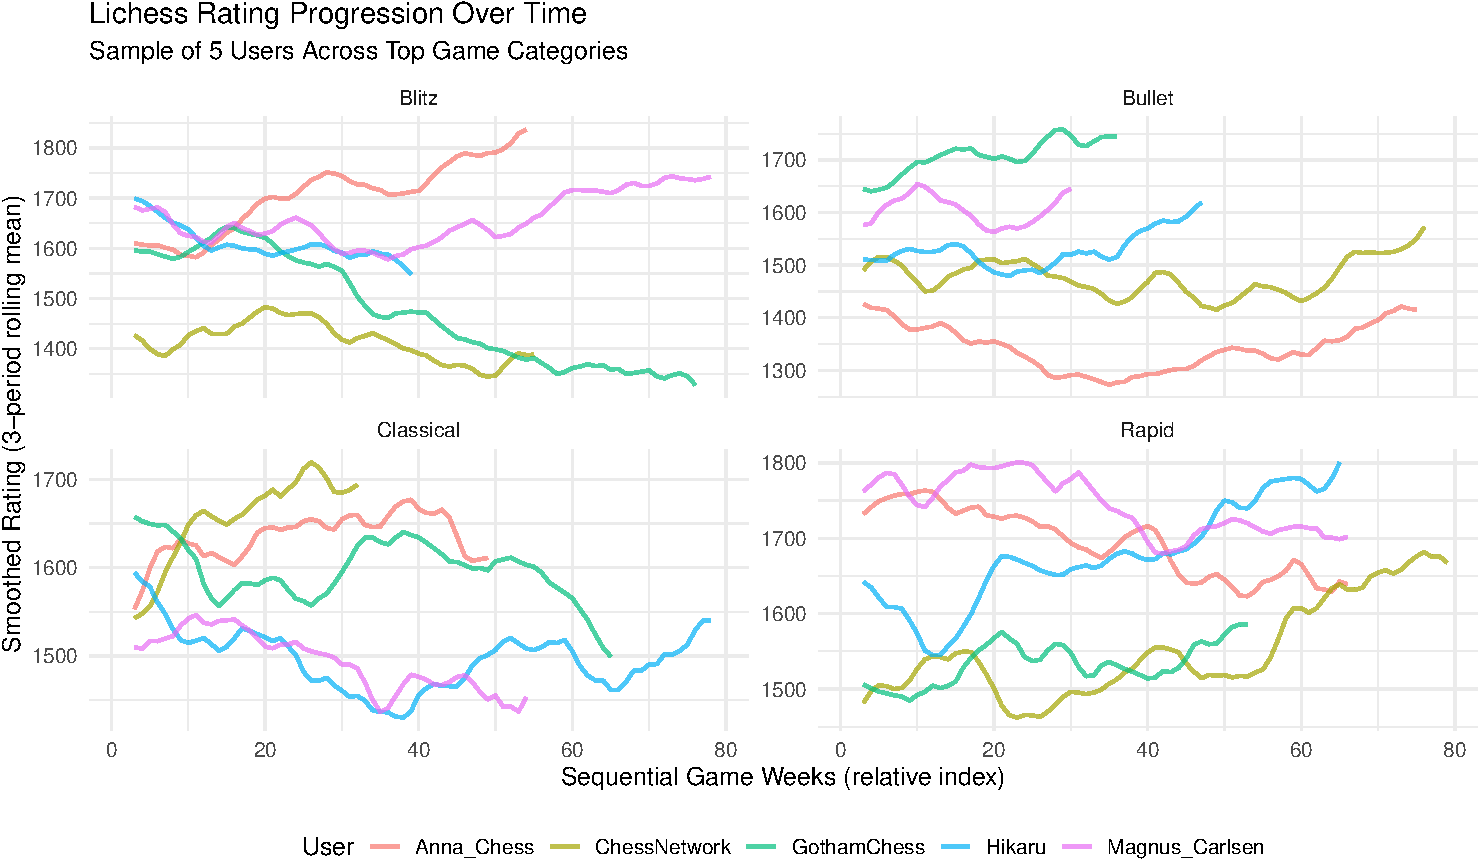
\includegraphics[keepaspectratio]{appendix_b_files/figure-latex/rating-time-series-1.pdf}}

\begin{quote}
\textbf{Interpretation:} Each panel tracks smoothed rating evolution for
a sample of users. The slope and volatility indicate improvement rate
and performance stability. Typical trends show plateauing after
\textasciitilde20--40 periods, reflecting rating convergence or skill
saturation.
\end{quote}

\begin{center}\rule{0.5\linewidth}{0.5pt}\end{center}

\subsubsection{B.4 Analytical
Highlights}\label{b.4-analytical-highlights}

\begin{itemize}
\tightlist
\item
  \textbf{Consistent upward trends} imply sustained learning and
  adaptation to faster time controls.
\item
  \textbf{Volatile fluctuations} correspond to periods of
  experimentation or inactivity.
\item
  Cross-category gaps (e.g., \emph{Blitz \textgreater{} Rapid
  \textgreater{} Classical}) align with expected behavioral rating
  hierarchies in online chess.
\item
  Aggregating trajectories could enable a \textbf{growth-rate model}
  (e.g., mixed-effects regression) quantifying individual improvement
  rates.
\end{itemize}

\begin{center}\rule{0.5\linewidth}{0.5pt}\end{center}

\subsubsection{B.5 Extension
Opportunities}\label{b.5-extension-opportunities}

\begin{enumerate}
\def\labelenumi{\arabic{enumi}.}
\tightlist
\item
  \textbf{Model Rating Growth:} Fit a linear or non-linear regression
  for each user to estimate weekly growth rate.
\end{enumerate}

\begin{Shaded}
\begin{Highlighting}[]
\NormalTok{model }\OtherTok{\textless{}{-}} \FunctionTok{lm}\NormalTok{(rating\_smooth }\SpecialCharTok{\textasciitilde{}}\NormalTok{ relative\_time, }\AttributeTok{data =}\NormalTok{ rating\_summary)}
\FunctionTok{summary}\NormalTok{(model)}
\end{Highlighting}
\end{Shaded}

\begin{verbatim}
## 
## Call:
## lm(formula = rating_smooth ~ relative_time, data = rating_summary)
## 
## Residuals:
##     Min      1Q  Median      3Q     Max 
## -5.6904 -2.4748 -0.0646  2.5959  5.6174 
## 
## Coefficients:
##                Estimate Std. Error t value Pr(>|t|)    
## (Intercept)   5.382e+00  2.380e-02 226.170  < 2e-16 ***
## relative_time 1.183e-04  3.413e-05   3.464 0.000533 ***
## ---
## Signif. codes:  0 '***' 0.001 '**' 0.01 '*' 0.05 '.' 0.1 ' ' 1
## 
## Residual standard error: 3.252 on 30421 degrees of freedom
##   (304 observations deleted due to missingness)
## Multiple R-squared:  0.0003943,  Adjusted R-squared:  0.0003615 
## F-statistic:    12 on 1 and 30421 DF,  p-value: 0.0005326
\end{verbatim}

\begin{enumerate}
\def\labelenumi{\arabic{enumi}.}
\setcounter{enumi}{1}
\item
  \textbf{Compare Variability by Rating Group:} Merge
  \texttt{rating\_summary} with the existing
  \texttt{player\_summary.csv} to test whether higher-rated players show
  less variance over time.
\item
  \textbf{Add Chess.com Parallel Data:} Use Chess.com's public API to
  collect equivalent histories and benchmark cross-platform consistency.
\end{enumerate}

\end{document}
